\documentclass[11pt, twoside, reqno]{book}
\usepackage{amssymb, amsthm, amsmath, amsfonts}
\usepackage{graphicx}
\graphicspath{ {images/} }
\usepackage[author-year]{amsrefs}
\usepackage{color}
\usepackage{hyperref}
\usepackage{verbatim}
\usepackage[title]{appendix}
\usepackage{pdfpages}
\usepackage{bardtex}

\styleoption{seniorproject}


\begin{document}

%For senior projects:
\titlepg{Don't Take This Personally: Sentiment Analysis for Identification of ``Subtweeting" on Twitter}{Noah Segal-Gould}
    {May}{2018}

\abstr

The purpose of this project is to identify subtweets. The Oxford English Dictionary defines ``subtweet" as a ``[Twitter post] that refers to a particular user without directly mentioning them, typically as a form of furtive mockery or criticism." This paper details a process for gathering a labeled ground truth dataset, training a classifier, and creating a Twitter bot which interacts with subtweets in real time. The Naive Bayes classifier trained in this project classifies tweets as subtweets and non-subtweets with an average $F_{1}$ score of 71\%. 

\tableofcontents

\dedic

I dedicate this senior project to @jack, who has willfully made numerous changes to Twitter which inevitably angered millions.

\acknowl

Thank you professors Sven Anderson, Keith O'Hara, and Rebecca Thomas for making this project possible through your combined efforts to teach and advise me. Thank you Benjamin Sernau '17 for enduring through three years of Computer Science courses with me and being a source of unending joy in my life. Thank you to Julia Berry '18, Aaron Krapf '18, and Zoe Terhune '18 for being my very best friends and giving me things worth caring about. Finally, thank you to my parents Tammy Segal and Emily Taylor for your constant support and patience throughout my four years at Bard College. 

\startmain


\intro

\textit{The data gathered for this project contains unsavory language which may be considered inappropriate.}

\section{Background}
\label{background}

This project utilizes the Twitter Application Programming Interface (API) as well as concepts from machine learning and text analysis. The ground truth dataset created for this project features 30,564 tweets by 27,711 unique users from March and April of 2018. There has been significant research in the field of sentiment analysis to identify the opinions held within bodies of text, however this research does not include so-called ``subtweets." The Oxford English Dictionary defines that a subtweet is a ``[tweet] that refers to a particular user without directly mentioning them, typically as a form of furtive mockery or criticism." Treated as a characteristic of a tweet's sentiment, we will utilize the Naive Bayes classification algorithm to perform sentiment analysis on subtweets.

For acquisition of a ground truth dataset, we consider \textbf{true subtweets} to be tweets to which another Twitter user replied who specifically called it out as a subtweet. We consider \textbf{true non-subtweets} to be tweets to which another user replied who specifically did \textbf{not} call it out as a subtweet. Consider these examples:

\begin{center}
	\begin{tabular}{ | p{2cm} | p{5cm} | p{5cm} | }
		\hline
		& True Subtweet Data& True Non-Subtweet Data
		\\ 
		\hline
		Tweet&Talk to him again about ``dropping me" and you'll get your teeth knocked out&That's been one of my biggest issues here; the onus is on ordinary people who, in their spare time, must campaign for the basic services of a city. This is not how progressive cities should be built 
		\\ 
		\hline
		Reply&Thomas don't subtweet me during work hours&i guess i am not as creative as i thought
		\\
		\hline
	\end{tabular}
\end{center}

We will keep these definitions and examples in mind when the classifier is used on original tweets independent of their replies. These will be called \textbf{predicted subtweets} and \textbf{predicted non-subtweets}. The following sections detail the resources and techniques utilized to acquire the labeled ground truth dataset, train the Naive Bayes classifier, and program a Twitter bot to interact with subtweets in real time.

\section{Changes in Data Acquisition}
\label{changes_in_data}

The novel approach developed for creating a ground truth dataset relied on a particular phenomenon in which Twitter users were already calling-out the subtweets of their peers. The following pattern was observed: a user would post a subtweet which was easily recognized by a peer, and that peer would then reply to that tweet in order to complain that the original user was subtweeting or to ask if the tweet was indeed a subtweet. Initially, the program used the Twitter API's search functionality to specifically search for replies to tweets which contained some form of the string ``subtweet." It utilized the API's status object to access the tweet to which it was replying. For two months, each day's alleged subtweets and their associated accusatory replies were saved.

Initially, the classifier was trained using a dataset which was half composed of these alleged subtweets and half composed of tweets randomly selected from a pre-labeled sentiment analyzed tweets dataset \cite{go_dataset}. This procedure failed to make the training data representative of \textbf{true subtweets} and \textbf{true non-subtweets}. The alleged subtweets downloading program was revised and it was set to download tweets with replies which specifically did \textbf{not} contain the string ``subtweet." In both the program which downloaded subtweets and the program which downloaded non-subtweets, the assumptions about these interactions would not hold true in every case. They were intended as generalizations which would make acquiring a ground truth dataset for use in performing binary classification significantly easier and less time-consuming than finding and labeling subtweets and non-subtweets by hand. Indeed, dataset utilized by Go et al. used a similar method for acquiring labeled data. In their \textit{Sentiment140} dataset, the labels were acquired according to emoticons present within the tweets instead of through hand-labeling by actual humans. 

\section{The Twitter API}
\label{twitter_api}

Twitter provides a free Application Programming Interface (API) to registered users and has done so since September of 2006 \cite{twitter_api_start}. The API allows developers to programmatically access and influence tweets individually or through real time search filters, and also read and write direct messages \cite{twitter_api_docs}. The creation of a Twitter application which utilizes the API requires creation and email verification of an account, and developers are also required to agree to the terms of service \cite{twitter_tos}. Creation of an application provides developers with authentication tokens which can then be used to access the API.

To make creation of Twitter applications easier, Tweepy \cite{tweepy_python} is an open source library for the Python programming language which provides methods and classes used to interact with the API and its status objects \cite{tweepy_status_object}. A Twitter status object is a dictionary of key and value pairs which contains text, media, and user information associated with particular tweets (i.e. statuses). There are rate limits for both reading and writing to the API which must be kept in mind when programming for it.

\section{Feature Extraction \& Selection}
\label{feature_extraction}

Feature extraction and selection are the processes by which text is modified prior to any kind of processing such that the important features within it are easily accessible. Changes are made to preserve the characteristics of the text which are relevant to the goal of the analysis and to leave out the ones which are irrelevant. Because we will be using Naive Bayes, we must keep in mind which features in each tweet (e.g. URLs and user names) ought to influence the probabilities that an entire feature-set (i.e. that whole tweet) suits a particular class.

\subsection{Regular Expressions}
\label{regular_expressions}

For text classification through machine learning, it is popular to modify the ground truth dataset to make features which are not important to the classification problem as \textbf{generic} as possible. For classification of subtweets, the classifier will treat URLs, mentions of usernames, and English first names generically. In other words, it will keep track of the existence of those features but specifically will not encounter the text contained within them. In identification of subtweets, there exists no syntactic or linguistic significance in the format of a URL or the name a user chooses to associate with themselves or another. However, the existence of those features within the tweet remains important. For this kind of substring searching, pattern matching through regular expressions was used to replace every occurence of URLs, usernames, and first names with special tokens which were not already in the dataset. The top 100 most common English names for both men and women over the last century were acquired from the United States Department of Social Security.

\subsection{Tokenization}
\label{tokenization}

Instead of training the classifier on entire strings, \textbf{tokenization} is necessary in order to extract individual features from the text. The Natural Language Toolkit (NLTK) provides a tweet tokenizer to achieve this. For some string, the tokenizer splits apart words, usernames, URLs, hashtags, and punctuating characters as individual tokens. NLTK's tweet tokenizer also appropriately distinguishes between punctuating characters and emoticons composed of punctuating characters.

\subsection{N-Grams}
\label{n_grams}

An \textbf{n-gram} is a contiguous sequence of $n$ tokens in a piece of text. For example, given a string such as ``This is a test," the bigrams ($n=2$) for this string are ``This is," ``is a," and ``a test." Instead of training the classifier using unigrams ($n=1$) exclusively, we train it using unigrams, bigrams, and trigrams ($n=3$). Thus, when the probability that some specific token within a tweet belongs to a specific class is calculated, its neighbors are also considered in combination with it. N-grams enable the classifier to treat particular groupings of tokens with some size $n$ as importantly as it treats the individual tokens, thus identifying particular word groupings most associated with the classes.

\subsection{Stop Words}
\label{stop_words}

A list of stop words typically contains the most common words in a language. For English text, the list is often composed of words such as ``the," ``it," and ``of." Tokens matching stop words are ignored during classifier training because they are too common to help the classifier distinguish subtweets from non-subtweets. 

\section{TF \& TF-IDF}
\label{tf_tf_idf}

The probabilities calculated for Naive Bayes are not best found using raw token counts within individual documents. Instead, TF-IDF is popularly used in order to vectorize the tokens for use in training the classifier. 

Term frequency (TF) is a simple method for vectorizing text in which all terms (i.e. tokens, features, words, etc.) in the corpus are featured in a vector for each document, and the frequency of each term is reflected in the number representing the corresponding term. The bag of words model essentially vectorizes features using this method. Unfortunately, TF falls short when the corpus of documents contains terms which appear frequently but do not necessarily help inform the classifier on terms that are best associated with a particular class. TF-IDF, or term frequency-inverse document frequency, is the product of the TF for a specific term and the inverse document frequency (IDF) for that same term. The TF is equal to the ratio between the number of occurrences of a term in a document, and the total number of words in that document. IDF, then, is the logarithm of the ratio between the number of documents in the corpus, and the number of documents which contain that term. Taking the logarithm means the value will be higher for rarer terms. Thus, the product of TF and IDF assigns weights which appropriately value terms which are frequent within a document but rare in the entire corpus of documents. Because the weighted feature vectors calculated using TF-IDF follow a multinomial distribution, our classification algorithm is specifically a Multinomial Naive Bayes classifier.

\section{Naive Bayes}
\label{naive_bayes}

Naive Bayes stands out as particularly simple and common for use in text classification. A \textbf{bag of words} model typically ignores word positions in favor of keeping track of raw token frequencies, which are weighted to produce TF-IDF feature vectors. Then, Bayes Theorem is utilized to predict the probability that a given feature set (e.g. words, sentences, etc.) belongs to a particular label (i.e. a category or class). Bayes theorem states the following:

\[\text{posterior probability}=\frac{\text{conditional probability} \cdot \text{prior probability}}{\text{evidence}}\] 

In all cases where we must calculate the probability for an entire feature-set, we simply take the product of all the extracted feature probabilities in the document. The \textbf{posterior probability} is the probability that a particular document belongs to a class given the observed features within that document. The Naive Bayes algorithm maximizes this probability in order to predict which class best fits a document. The \textbf{conditional probability} refers to the likelihood of encountering the features within a document given that those features belong to a particular class. The \textbf{prior probability} is otherwise known as the \textbf{class probability} and is equal to the general probability of encountering a particular class. In our case, we have chosen to keep our classes balanced (i.e. there are equal numbers of documents in both), so the prior probability will always be 50\%. The evidence, then, refers to the probability of encountering the features within a document \textbf{independent} of the class label. It is often ignored in the final classification step on the basis that it acts merely as a scaling factor when trying to maximize which class produces the greater posterior probability. Consider this classification example:
\[
\begin{split} 
	& \text{if } P(  \omega = \text{subtweet} \mid \textbf{x}) \ge P(\omega = \text{non-subtweet} \mid \textbf{x})  \text{ classify as subtweet, }\\
	&  \text{else classify as non-subtweet. }
\end{split}
\]

\noindent 
Dropping the evidence term on the basis that it is constant for both classes, we expand that:
\[
\begin{split} 
	&  P(\omega = \text{subtweet} \mid \textbf{x}) = P(\textbf{x} \mid \omega = \text{subtweet}) \cdot P(\text{subtweet}) \\
	&  P(\omega = \text{non-subtweet} \mid \textbf{x}) = P(\textbf{x} \mid \omega = \text{non-subtweet}) \cdot P(\text{non-subtweet})
\end{split} 
\]

\noindent
Assuming the posterior probability for the former is greater than or equal to the latter, the classifier predicts that the document fits that class. The naive assumption maintains that all features are treated as conditionally independent (i.e. that the presence or omission of a particular feature does not change the likelihood of encountering other features), and although this is frequently violated, Naive Bayes often performs well anyway \cite{naive_bayes_optimality}. 

For cases in which the classifier encounters a feature absent from the features which were used to train it, a so-called \textbf{zero probability} appears. Because the probability of encountering the feature is 0, \textbf{additive smoothing} is often utilized to appropriately weight new features using an extra term $\alpha$, so the probability that an entire feature-set fits into a specific class is not 0. In this project, we use \textbf{Laplace smoothing} ($\alpha=1$). This technique smooths categorical data by including the pseudo-count $\alpha$ into each probability estimate. Thus, the probability of a feature given a particular class becomes:

\[P(x_i \mid \omega_j) = \frac{N_{x_i, \omega_j}+\alpha}{N_{\omega_j} + \alpha \, d}  \quad (i = (1, ... , d))\]

\noindent 
where $N_{x_i, \omega_j}$ is the number of times feature $x_i$ appears in samples from class $\omega_j$, $N_{\omega_j}$ is the total count of all features in class $\omega_j$, $\alpha$ is the parameter for additive smoothing, and $d$ is the dimensionality of the feature vector $\textbf x = [x_1, ..., x_d]$. Compared to datasets which contain millions of tweets such as \textit{Sentiment140} \cite{go_dataset}, our classifier has access to significantly fewer documents. We utilize Laplace smoothing because when the classifier is tested on new tweets it will likely encounter never before seen features given the limited size of the ground truth dataset.

\section{K-Folds Cross-Validation}
\label{cross_validation}

Instead of using the entire ground truth dataset as training data for the Naive Bayes classifier, we can split it apart into a \textbf{training set} and a \textbf{test set}. The training set is fed to the classifier, and the test set is used to observe statistics about its performance. In cross-validation using $k$-folds, we make random splits in the dataset $k$ times to create several training set and test set sections. We then take statistical measurements of how well the classifier performs on the testing set for each fold. If we made one single split into training and testing sections of our ground truth dataset and only used that single testing set to gather statistics on the classifier's performance, we would not be able to confirm that those statistics were representative of all the data in the entire ground truth dataset. Instead, we perform 10-fold cross validation, choosing 90\% of the data to be the training set, and 10\% to be the testing set in each fold. Precision, $F_{1}$ score, and recall are calculated within each iteration of the 10 folds, thus utilizing 10 different test datasets. Finally, we use the averages of those statistics across all folds to measure the overall performance of the classifier. The following figure illustrates this process:

\begin{figure}[h]
	\centering
	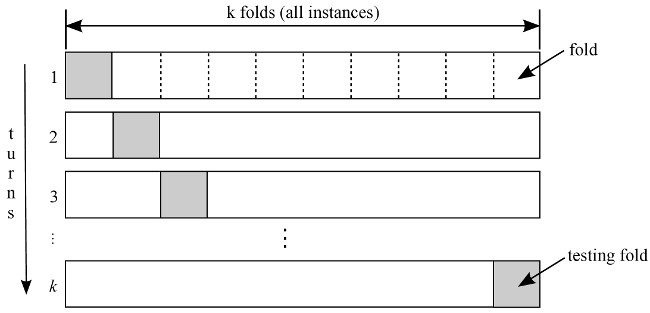
\includegraphics{k_folds}
	\caption{K-Folds Cross-Validation Example \cite{k_folds}}
	\label{fig:k_folds}
\end{figure}

\section{Statistical Considerations}
\label{statistical_considerations}

In the binary classification of subtweets and non-subtweets, we consider true positives (TP) to be true subtweets which were correctly labeled as predicted subtweets, false positives (FP) to be true non-subtweets which were incorrectly labeled as predicted subtweets, true negatives (TN) to be true non-subtweets which were correctly labeled as predicted non-subtweets, and false negatives (FN) to be true subtweets which were incorrectly labeled as predicted non-subtweets. As such, there are two ways for the classifier to be wrong: it can produce false negatives and false positives.

\subsection{Precision}
\label{precision}

Precision refers to the ratio between the true positives, and the true positives and false positives. It is also known as the positive predictive value.

\[P=\frac{TP}{TP+FP}\] 

\subsection{Recall}
\label{recall}

Recall, then, refers to the ratio between the number of true positives, and the true positives and false negatives. It is also known as the sensitivity.

\[R=\frac{TP}{TP+FN}\] 

\subsection{Accuracy}
\label{accuracy}

The accuracy is the ratio between the true positives and the true negatives, and the true positives, true negatives, false positives, and false negatives. Accuracy alone is a particularly bad quantifier of how well a classifier performs when working with data which is class-imbalanced (i.e. there are not equal numbers of items in each class). In our ground truth dataset, the classes are balanced so measuring accuracy will still be informative.

\[A=\frac{TP+TN}{TP+TN+FP+FN}\] 

\subsection{F1 Score}
\label{f1_score}

The $F_{1}$ score is a weighted average of the precision and recall. Thus, it takes both false positives and false negatives into account.

\[F1=\frac{2*(P*R)}{P+R}\] 

\subsection{Null Accuracy}
\label{null_accuracy}

The null accuracy is just the accuracy which is obtained by always predicting the most frequent class. Because there are two classes and the tweets within the ground truth dataset equally compose both, the null accuracy will always be 50\%.

\section{Review of Literature}
\label{review_of_literature}

``Subtweet" was coined in December of 2009 by Twitter user Chelsea Rae \cite{first_subtweet} and was entered into Urban Dictionary the following August \cite{urban_dictionary}. In ``To tweet or ‘subtweet’?: Impacts of social networking post directness and valence on interpersonal impressions" \cite{subtweets_communications}, Edwards and Harris sought to analyze student participants' perceptions of known subtweeters. In the news, too, subtweets have garnered attention in \textit{The Atlantic} \cite{the_atlantic}, \textit{The Washington Post} \cite{the_washington_post}, and \textit{Slate} \cite{slate}. In news media, subtweets garner attention for their prevalence among government officials as well. Following President Donald Trump's inauguration, The Washington Post compiled its ``A running list of all the possible subtweets of President Trump from government Twitter accounts," \cite{the_washington_post_trump} cementing subtweets as particularly newsworthy.

There were over 140 million active Twitter users who sent 340 million text-based tweets to the platform every day by March of 2012 \cite{twitter_stats}. Since Twitter-founder Jack Dorsey sent the first Tweet in March of 2006 \cite{first_tweet} social scientists, political scientists, and computer scientists have applied machine learning techniques to understand the patterns and structures of the conversations held on the platform. Through sentiment analysis, we are able to use machine learning to identify patterns within natural language which indicate particular feelings both broadly (e.g. positive, neutral, or negative) and toward topics (e.g. politics, terrorism, brands, etc.).

On Twitter, the most common way to publicly communicate with another user is to compose a tweet and place an ``@" before the username of that user somewhere in the tweet (e.g. "How are you doing, @NoahSegalGould?"). Through this method, public discussions on Twitter maintain a kind of accountability: even if one were to miss the notification that they were mentioned in a tweet, one's own dashboard keeps a running list of their most recent mentions. 

If an individual sought to disparage or mock another, they could certainly do so directly. But the targeted user would probably notice, and through the search functions of the platform, anyone could see who has mentioned either their own or another's username. Instead, a phenomenon persists in which users of the platform deliberately insult others in a vague manner by making complaints while omitting the targets of those complaints. 

Although the OED's definition states that a subtweet ``...refers to a particular user without directly mentioning them, typically as a form of furtive mockery or criticism," it is perhaps too restrictive. Some individuals believe subtweets abide by this definition, but others expand it to allow inclusion of others' real names (especially if that individual does not own a Twitter account), and some do not even require that a particular user be the target of the tweet. Because subtweeting is colloquial in nature, we will expand the definition of subtweet to permit these less restrictive features.

Sentiment analysis on social networking services such as Twitter has garnered attention within seemingly distinct fields of interest. In ``Text mining for market prediction: A systematic review," Nassirtoussi et al. surveyed varied methods for text-mining social media for sentiment analysis of financial markets and approached that problem with both behavioral and economic considerations in mind \cite{sentiment_analysis_markets}. Following a terrorist event in Woolwich, London in 2013, Burnap et al. analyzed the immediate Twitter response following the attack to inform statistics on how long it takes for responses from official sources to disseminate during crises \cite{sentiment_analysis_terrorism}. Prior research of these kinds utilizes sentiment analysis techniques on tweets, but no known research exists which specifically performs any sentiment analysis on subtweets. 

Long before Twitter, psychologist Gordon Allport wrote about ``antilocution" in \textit{The Nature of Prejudice} \cite{antilocution}. For Allport, antilocution was the first of several degrees of apathy which measure prejudice in a society. It represented the kind of remarks which target a person, group, or community in a public or private setting but do not address the targeted individual directly. Different from both hate speech and subtweeting, antilocution necessitates that an in-group ostracize an unaware out-group through its biases.

The most germane research available focuses on sentiment analysis of figurative language. Determining sentiment based on features of text which are distinctly separate from their literal interpretations presents difficulties for human readers as well as computer programs. In \textit{SemEval}, the International Workshop on Semantic Evaluation, analysis of figurative language on Twitter has been a core task for their competition since 2015 \cite{semeval_2015} and returns this year with a specific focus on ironic tweets \cite{semeval_2018}. In this year's description for ``Task 3: Irony detection in English tweets," Van Hee et al. touch upon online harassment as a potential point of significance for sentiment analysis of ironic tweets.  

We pursue sentiment analysis of subtweets in order to challenge the hypocrisy of utilizing a service which presents itself as a public forum to speak in distinctly private ways. Toward this end, these are our goals: this project will provide a framework for collecting examples of subtweets, train a classification algorithm using those examples, and finally utilize that classifier in real time to make tweets which were intended to be unseen by specific parties easily accessible to all parties. In presenting covertly hurtful content as obviously hurtful in a public fashion, perhaps it will promote a particular awareness that tweets posted by public accounts are indeed publicly accessible, and that Twitter's Terms of Service \cite{twitter_tos} allows for this kind of monitoring. 

Using a machine-learning approach to perform sentiment analysis, syntactic and linguistic features are typically utilized in probabilistic (e.g. Naive Bayes and Maximum Entropy) and linear (e.g. Support Vector Machines and Neural Networks) classification algorithms. The probabilistic approach is sometimes called \textit{generative} because such models generate the probabilities of sampling particular terms \cite{sentiment_survey}. Linear classification utilizes the vectorized feature space of words, sentences, or documents to find a separating hyperplane between multiple classes. In this project, we approach the problem of identifying subtweets using the probabilistic Naive Bayes classification algorithm.

\chapter{Implementation}
\label{implementation}

Given access to the Twitter API, the programs developed for this project can download a ground truth dataset of \textbf{true subtweets} and \textbf{true non-subtweets}, clean the data and select its features, train a Naive Bayes classifier using that dataset, and interact with \textbf{predicted subtweets} in real time. The following sections are sequentially ordered and contain brief explanations of the process at each step.

\section{Searching for Tweets Using the Twitter API}
\label{searching_with_api}

The first step in this process is to acquire data for the ground truth dataset. After loading our API credentials we use the following code to acquire tweets with replies which \textbf{do} and \textbf{do not} call them out as subtweets:

[Show code and explain how searching works with Tweepy.]

\section{Cleaning the Data}
\label{cleaning_data}

[Show code and explain how text cleaning genericizes certain features and ignores tweets lacking enough English words.]

\section{Training the Classifier}
\label{training_and_k_folds}

[Explain how pipelines are trained and how K-Folds splits the dataset.]

\chapter{Results}
\label{results}

\section{Ground Truth Dataset}
\label{ground_truth_dataset}

[Explain the tables and figures.]

\section{Confusion Matrices}
\label{confusion_matrices}

A confusion matrix is a table which visualizes the performance of an algorithm. In this case, I implemented a Naive Bayes classifier from Scikit Learn on my dataset and included in my results is a confusion matrix of the performance...

[Explain how to read a confusion matrix and show the test and training figures.]

\section{Statistical Analyses}
\label{statistical_analyses}

\section{Application of the Classifier on Tweets from Known Subtweeters}
\label{known_subtweeters_analysis}

\section{Most Informative Features}
\label{most_informative_features}

[Explain how to read the most informative features for each class (or just the "subtweet" class) and show the table.]

[Show the scores from K-Folds.]

\section{The Twitter Bot}
\label{the_twitter_bot}

[Explain how the Twitter bot works and show code as well as examples of interactions.]

\section{Discussion}
\label{discussion}

[Discussion of results.]

\chapter{Conclusion}
\label{conclusion}

\section{Summary of Project Achievements}
\label{summary}

[Ground truth data, classifier, cleaning, Twitter bot.]

\section{Future Work \& Considerations}
\label{future_work_and_considerations}

[Test other classification algorithms. Utilize more training data.]

\begin{bibliog}

\bib{twitter_stats}{article}{
	author={Twitter},
	title={Twitter turns six},
	date={2012},
	eprint={https://blog.twitter.com/official/en_us/a/2012/twitter-turns-six.html},
}

\bib{first_tweet}{article}{
	author={Dorsey, Jack},
	title={inviting coworkers},
	date={2006},
	eprint={https://twitter.com/jack/status/29},
}

\bib{twitter_tos}{article}{
	author={Twitter},
	title={Twitter Terms of Service},
	date={2016},
	eprint={https://twitter.com/en/tos}
}

\bib{antilocution}{article}{
	title={The nature of prejudice},
	author={Allport, Gordon W},
	date={1954}
}

\bib{first_subtweet}{article}{
	author={Rae, Chelsea},
	title={I hate when i see people...},
	date={2009},
	eprint={https://twitter.com/Chelsea_x_Rae/status/6261479092},
}

\bib{urban_dictionary}{article}{
	author={Urban Dictionary},
	title={Subtweet},
	date={2010},
	eprint={https://www.urbandictionary.com/define.php?term=subtweet},
}

\bib{subtweets_communications}{article}{
	author={Edwards, Autumn},
	author={Harris, Christina~J},
	title={To tweet or ‘subtweet’?: Impacts of social networking post directness and valence on interpersonal impressions},
	date={2016},
	journal={Computers in Human Behavior},
	volume={63},
	pages={304\ndash 310},
}

\bib{the_atlantic}{article}{
	author={Madrigal, Alexis~C.},
	title={Behind the machine's back: How social media users avoid getting turned into big data},
	date={2014},
	eprint={https://goo.gl/h36jxx},
}

\bib{the_washington_post}{article}{
	author={Dewey, Caitlin},
	title={Study confirms what you always knew: People who subtweet are terrible},
	date={2016},
	eprint={https://goo.gl/SeV3mx},
}

\bib{slate}{article}{
	author={Hassler, Chelsea},
	title={Subtweeting looks terrible on you. (you know who you are.)},
	date={2016},
	eprint={https://goo.gl/NCz27z},
}

\bib{the_washington_post_trump}{article}{
	author={Ohlheiser, Abby},
	title={A running list of all the possible subtweets of President Trump from government Twitter accounts},
	date={2017},
	eprint={https://goo.gl/hFh81R},
}

\bib{hateful_conduct}{article}{
	author={Twitter},
	title={Hateful conduct policy},
	date={2018},
	eprint={https://help.twitter.com/en/rules-and-policies/hateful-conduct-policy},
}

\bib{sentiment_analysis_markets}{article}{
	author={Nassirtoussi, Arman~Khadjeh},
	author={Aghabozorgi, Saeed},
	author={Wah, Teh~Ying},
	author={Ngo, David Chek~Ling},
	title={Text mining for market prediction: A systematic review},
	date={2014},
	journal={Expert Systems with Applications},
	volume={41},
	number={16},
	pages={7653\ndash 7670},
}

\bib{sentiment_analysis_terrorism}{article}{
	author={Burnap, Pete},
	author={Williams, Matthew~L},
	author={Sloan, Luke},
	author={Rana, Omer},
	author={Housley, William},
	author={Edwards, Adam},
	author={Knight, Vincent},
	author={Procter, Rob},
	author={Voss, Alex},
	title={Tweeting the terror: modelling the social media reaction to the woolwich terrorist attack},
	date={2014},
	journal={Social Network Analysis and Mining},
	volume={4},
	number={1},
	pages={206},
}

\bib{semeval_2015}{article}{
	title={Semeval-2015 task 11: Sentiment analysis of figurative language in twitter},
	author={Ghosh, Aniruddha},
	author={Li, Guofu}, 
	author={Veale, Tony},
	author={Rosso, Paolo}, 
	author={Shutova, Ekaterina}, author={Barnden, John}, 
	author={Reyes, Antonio},
	journal={Proceedings of the 9th International Workshop on Semantic Evaluation (SemEval 2015)},
	pages={470\ndash478},
	year={2015}
}

\bib{semeval_2018}{article}{
	author={Van Hee, Cynthia}, 
	author={Lefever, Els}, 
	author={Host, Véronique},
	title={Semeval-2018 Task 3: Irony detection in English Tweets},
	date={2018},
	journal={Proceedings of the 12th International Workshop on Semantic Evaluation (SemEval-2018)}
}

\bib{sentiment_survey}{article}{
	title={Sentiment analysis algorithms and applications: A survey},
	author={Medhat, Walaa},
	author={Hassan, Ahmed},
	author={Korashy, Hoda},
	journal={Ain Shams Engineering Journal},
	volume={5},
	number={4},
	pages={1093\ndash1113},
	date={2014},
}

\bib{naive_bayes_optimality}{article}{
	title={The optimality of naive Bayes},
	author={Zhang, Harry},
	journal={AA},
	volume={1},
	number={2},
	pages={3},
	date={2004}
}

\bib{go_dataset}{article}{
	title = {Twitter Sentiment Classification using Distant Supervision},
	author = {Go, Alec},
	author = {Bhayani, Richa},
	author = {Huang, Lei},
	journal = {CS224N Project Report, Stanford},
	pages = {12},
	date = {2009}
}

\bib{twitter_api_start}{article}{
	author={Stone, Biz},
	title={Introducing the Twitter API},
	date={2006},
	eprint={https://blog.twitter.com/official/en_us/a/2006/introducing-the-twitter-api.html},
}

\bib{twitter_api_docs}{article}{
	author={Twitter},
	title={Twitter API Docs},
	date={2018},
	eprint={https://developer.twitter.com/en/docs},
}

\bib{tweepy_python}{article}{
	title={tweepy Documentation},
	author={Roesslein, Joshua},
	eprint={http://docs.tweepy.org/en/v3.5.0/},
	volume={5},
	date={2009}
}

\bib{tweepy_status_object}{article}{
	author={Twitter},
	title={Tweet objects},
	date={2018},
	eprint={https://developer.twitter.com/en/docs/tweets/data-dictionary/overview/tweet-object},
}

\bib{k_folds}{article}{
	author={Borovicka, Tomas},
	author={Jirina Jr, Marcel},
	author={Kordik, Pavel},
	author={Jirina, Marcel},
	title={Selecting representative data sets},
	date={2012}
}

\end{bibliog}

\end{document}

% end of file bardproj_template.tex
